\section{Results}\label{sec:results}
In this section I report the outcomes from the main linked sample
described in section \ref{sec:data-IPUMS} 
and estimated coefficients from section \ref{sec:wage-reg}.

\begin{table}[htbp]
   \caption{\label{tbl:reg1} Earning effects of internment}
   \bigskip
   \centering
   \begin{tabular}{lcccc}
      \toprule
       & \multicolumn{4}{c}{Income in 1950}\\
                                   & (1)     & (2)             & (3)             & (4)\\  
      \midrule 
      Internment Status            & -42.07  & 232.4$^{***}$   & 250.7$^{***}$   & 80.90\\   
                                   & (36.02) & (60.49)         & (59.86)         & (91.11)\\   
      Age                          &         & 33.30$^{***}$   & 12.45           & 11.22$^{**}$\\   
                                   &         & (7.837)         & (8.210)         & (4.786)\\   
      Age square                   &         & -0.5353$^{***}$ & -0.3143$^{***}$ & -0.3024$^{***}$\\   
                                   &         & (0.0808)        & (0.0835)        & (0.0461)\\   
      Male                         &         & 645.4$^{***}$   & 487.5$^{***}$   & 488.3$^{***}$\\   
                                   &         & (33.47)         & (35.14)         & (17.22)\\   
      Japanese                     &         & -210.0$^{***}$  & -246.2$^{***}$  & -98.45\\   
                                   &         & (63.93)         & (64.55)         & (88.69)\\   
      Income in 1940               &         &                 & 0.2409$^{***}$  & 0.2334$^{***}$\\   
                                   &         &                 & (0.0189)        & (0.0218)\\   
       \\
      Standard-Errors & \multicolumn{3}{c}{IID} & State$_{1940}$ \\ 
      Observations                 & 8,136   & 8,136           & 8,136           & 8,136\\  
      R$^2$                        & 0.00017 & 0.07616         & 0.10227         & 0.10882\\  
      Within R$^2$                 &         &                 & 0.08326         & 0.07855\\  
       \\
      Education fixed effects      &         &                 & $\checkmark$    & $\checkmark$\\   
      State$_{1940}$ fixed effects &         &                 &                 & $\checkmark$\\   
      \bottomrule
   \end{tabular}
\end{table}

Table \ref{tbl:reg1} presents the correlation between my predicted internment status and income in 1950.
All income amounts are reported in 1950 dollars.
Column (1) shows that on average, internees' incomes were 42 dollars lower than non-internees 
but that this effect is not statistically significant at the 10\% confidence level.
However, there is reason to believe that this estimate does not reflect the true causal effect of internment on later earnings.
For example, the Japanese living outside the West Coast may have already been a group that was self-selected for higher income mobility.
Additionally, if Japanese experienced higher post-war discrimination than Chinese during this period,
then this correlation will be a downward-biased estimate of the true effect of internment status itself when compared with the 
mostly Chinese control group.

To address these concerns, columns (2) through (4) 
add additional controls from equation \ref{eq:mainreg}.
When I include demographic controls in column (2) 
including respondents' sex, race, and a quadratic in age,
the coefficient on the predicted internment status increases 
to a statistically significant positive effect of \$234.
At the average 1950 wage for Japanese of \$1,004, 
this represents about a 20\% increase in wages by internees,
relative to their counterfactual outcomes.
Because Japanese and Chinese populations were similar in age and sex
distributions at this time,
this seems to provide evidence that the differences in labor market 
discrimination between Japanese and Chinese in 1950
are causing a difference in the correlation in column (1) 
and the coefficient on internment status in column (2).

Column (3) includes additional controls for an individual's 
pre-internment income and their level of education.
While the main coefficient on internment status remains similar,
a Wald test rejects the null hypothesis
that the coefficient on 1940 income is zero
at the 95\% confidence level.
By controlling for an individual census respondent's level of income
prior to any internment policies,
this specification helps to address potential concerns
that higher-earning Japanese who were living on the West Coast in 1940
may have had an easier time escaping internment through voluntary migration
but would appear as treated based on their original 1940 county of residence.

Within the West Coast states, 
the majority of the Japanese population lived in California in 1940.
It is possible that due to selection or ethnic enclave effects 
\citep{edinEthnicEnclavesEconomic2003},
Californian internees may have experienced higher income growth
compared to internees from Arizona, Oregon, or Washington.
Column (4) adds fixed-effects to account for the effect of internment on wage effects to
differ by their state of residence in 1950.
After allowing for internees coming from different states
to have different intercepts in equation \ref{eq:mainreg},
I can no longer reject the null hypothesis that 
internees from higher internment proportions within the same state
experienced any significantly higher wages in 1950 
than those from less intensively interned counties.

\subsection{Alternative Internment Measures}\label{sec:altint}

Table \ref{tbl:reg_altint} shows the estimates of equation \ref{eq:mainreg}
using three additional estimating methods for $\hat{E}[I_i]$.
These methods condition on different subsets of the variables
$state$ or $county$ of individual $i$ in 1940;
as well as their birth year, $byr$; birthplace, $bpl$; $sex$; and $race$.

\begin{table}[htbp]
   \caption{\label{tbl:reg_altint} Estimated effects using alternate internment prediction methods}
   \bigskip
   \centering
   \begin{tabular}{lcccc}
      \toprule
       & \multicolumn{4}{c}{Income in 1950}\\
                                                & (1)             & (2)             & (3)             & (4)\\  
      \midrule 
      $\hat{E}[I|county,race]$                  & 250.7$^{***}$   &                 &                 &   \\   
                                                & (59.86)         &                 &                 &   \\   
      Age                                       & 12.45           & 12.78           & 13.00           & 13.04\\   
                                                & (8.210)         & (8.221)         & (8.210)         & (8.210)\\   
      Age square                                & -0.3143$^{***}$ & -0.3189$^{***}$ & -0.3236$^{***}$ & -0.3237$^{***}$\\   
                                                & (0.0835)        & (0.0836)        & (0.0835)        & (0.0835)\\   
      Male                                      & 487.5$^{***}$   & 485.0$^{***}$   & 486.1$^{***}$   & 499.5$^{***}$\\   
                                                & (35.14)         & (35.17)         & (35.13)         & (35.30)\\   
      Japanese                                  & -246.2$^{***}$  & -44.20          & -268.6$^{***}$  & -208.1$^{***}$\\   
                                                & (64.55)         & (39.78)         & (66.73)         & (56.02)\\   
      Income in 1940                            & 0.2409$^{***}$  & 0.2416$^{***}$  & 0.2391$^{***}$  & 0.2406$^{***}$\\   
                                                & (0.0189)        & (0.0189)        & (0.0189)        & (0.0189)\\   
      $\hat{E}[I|county]$                       &                 & 2,041.8         &                 &   \\   
                                                &                 & (1,284.3)       &                 &   \\   
      $\hat{E}[I_i|state, bpl, byr, race]$      &                 &                 & 282.5$^{***}$   &   \\   
                                                &                 &                 & (64.33)         &   \\   
      $\hat{E}[I|county, sex, bpl, byr, race]$  &                 &                 &                 & 213.7$^{***}$\\   
                                                &                 &                 &                 & (48.55)\\   
       \\
      Observations                              & 8,136           & 8,136           & 8,136           & 8,136\\  
      R$^2$                                     & 0.10227         & 0.10061         & 0.10246         & 0.10247\\  
      Within R$^2$                              & 0.08326         & 0.08156         & 0.08346         & 0.08346\\  
       \\
      Education fixed effects                   & $\checkmark$    & $\checkmark$    & $\checkmark$    & $\checkmark$\\   
      \bottomrule
   \end{tabular}
\end{table}

Column (1) reports the same estimate as the main regression result
in table \ref{tbl:reg1} using $\hat{E}[I|county, race]$
as the estimated internment status conditional on county of residence and race.
Column (2) removes $race$ as a variable to predict internment,
applies the county-level ratio of internees to 1940 Japanese population
for both the Japanese and Chinese residents of each county.
Although the estimate of $\hat{E}[I]$ on income in 1950 
is much larger in magnitude than the equivalent estimate in Column (1),
the standard error on this estimate is also much larger
such that we cannot reject the null that county-level internment proportion alone
has a positive effect on income.
Because this county internment proportion
does not seem to explain any significant gap in income
when separately conditioning on individual race,
there seems to be evidence that the intersection of Japanese individuals
coming from more highly interned counties is in fact a relevant factor.
This evidence seems to contradict the possibility that something about the
highly interned counties themselves were also benefitting the Chinese individuals
who came from those counties.

Column (3) is the internment probability used by \cite{arellano-boverDisplacementDiversityMobility2022},
and instead of $county\times race$ level internment status,
it uses $\textbf{state}$-level internment proportions
together with birthplace and birthyear categories of internees
to predict individual internment status.
Although the estimate of internment on income is slightly larger here
than in column (1),
The overall magnitude and level of significance are similar.
In column (4), when conditioned on county and the full set of demographics,
the estimated effect $\hat{\beta}$  is slightly lower,
but again of similar magnitude and significance level.

By comparing column (1) to columns (3) and (4),
there does not appear to be much additional explanatory power gained 
by including additional demographic factors in $\hat{E}[I]$ besides race.

For these reasons, I use $\hat{E}[I|county, race]$
as the predicted internment status in the other empirical specifications
in this paper.


\subsection{Difference-in-differences estimates}

Table \ref{tbl:regdid} shows the difference-in-differences estimates
from a regression with the general formula:

\begin{equation}\label{eq:didreg}
  Y_i = \alpha + \beta \hat{E}[I_i]\times\mathbb{I}(YEAR=1950) 
        + \mathbb{X}_i \Gamma + \epsilon_i
\end{equation}.

For my sample, there are only two time periods: 1940 and 1950.
This regression also includes education levels and a quadratic function of age
as the only time-varying controls.
Unlike the main regression specification which allows for each linked individual
to have a different trend in incomes by comparing against their own 1940 income,
this specification only captures the difference-in-differences for the overall
groups defined by their treatment status.

\begin{table}[htbp]
   \caption{\label{tbl:regdid} Difference-in-difference regression estimates}
   \bigskip
   \centering
   \begin{adjustbox}{width = \textwidth, center}
      \begin{tabular}{lccc}
         \toprule
          & \multicolumn{3}{c}{INCWAGE}\\
                                                                      & (1)             & (2)             & (3)\\  
         \midrule 
         age\_adj                                                     & 63.13$^{***}$   & 64.15$^{***}$   & 61.45$^{***}$\\   
                                                                      & (4.828)         & (4.719)         & (4.291)\\   
         age\_adj square                                              & -0.7427$^{***}$ & -0.7534$^{***}$ & -0.7186$^{***}$\\   
                                                                      & (0.0494)        & (0.0486)        & (0.0461)\\   
         YEAR1940 $\times$ $\hat{E}[I|county,race]$                   & -404.2$^{***}$  &                 &   \\   
                                                                      & (46.48)         &                 &   \\   
         YEAR1950 $\times$ $\hat{E}[I|county,race]$                   & 193.6$^{***}$   &                 &   \\   
                                                                      & (59.50)         &                 &   \\   
         YEAR1940 $\times$ $\hat{E}[I_i|state, bpl, byr, race]$       &                 & -395.8$^{***}$  &   \\   
                                                                      &                 & (49.82)         &   \\   
         YEAR1950 $\times$ $\hat{E}[I_i|state, bpl, byr, race]$       &                 & 210.9$^{***}$   &   \\   
                                                                      &                 & (60.80)         &   \\   
         YEAR1940 $\times$ $\hat{E}[I|county, sex, bpl, byr, race]$   &                 &                 & -348.3$^{***}$\\   
                                                                      &                 &                 & (39.67)\\   
         YEAR1950 $\times$ $\hat{E}[I|county, sex, bpl, byr, race]$   &                 &                 & 191.6$^{***}$\\   
                                                                      &                 &                 & (35.00)\\   
          \\
         Observations                                                 & 16,272          & 16,272          & 16,272\\  
         R$^2$                                                        & 0.08263         & 0.08187         & 0.10987\\  
         Within R$^2$                                                 & 0.05989         & 0.05911         & 0.05029\\  
          \\
         EDUCD fixed effects                                          & $\checkmark$    & $\checkmark$    & $\checkmark$\\   
         State fixed effects                                          &                 &                 & $\checkmark$\\   
         County fixed effects                                         &                 &                 & $\checkmark$\\   
         \bottomrule
      \end{tabular}
   \end{adjustbox}
\end{table}

Table \ref{tbl:regdid} shows the estimates of this regression across
the three different predictions of internment status described in \ref{sec:altint}.
Similar to the results of the main regression, the different estimates
of $\hat{\beta}$ do not vary by much between the three versions of $\hat{E}[I]$.
The estimated effect, between \$190 and \$250, also matches the
magnitude of the estimates from earlier specifications.

\subsection{Mechanisms}

Due to the surprising nature of the result above 
that interned Japanese experienced higher incomes in 1950,
in the following sections I examine some of the potential mechanisms
that might have contributed to the main finding.

\subsubsection{Occupation and employment}

One explanation for internment having a seemingly positive effect on income
is that Japanese internees who lost savings or property may have adapted
by increasing their participation in formal labor that paid wages
(instead of earnings from working their own farms, businesses, etc).

Table \ref{tbl:reg2} reports the estimated effects of internment status
on an indicator of whether an individual was employed in 1950,
the number of hours they reported working last week,
the number of weeks worked in the last year,
an occupational ranking based on the median earnings in their reported occupation category,
and an indicator for whether they reported a different occupation from their 1940 one.

\begin{table}[htbp]
   \caption{\label{tbl:reg2} Employment and occupation effects}
   \begin{adjustbox}{width = \textwidth, center}
      \begin{tabular}{lccccc}
         \toprule
                               & Employed        & Hours worked    & Weeks worked    & Occ. score      & Occ. change\\  
                               & (1)             & (2)             & (3)             & (4)             & (5)\\  
                               &  Logit          & OLS             & OLS             & OLS             & Logit\\  
         \midrule 
         % (Intercept)           & -3.402$^{***}$  & -4.282          & 6.322$^{***}$   & 13.05$^{***}$   & -1.898$^{***}$\\   
         %                       & (0.2640)        & (3.084)         & (1.029)         & (2.171)         & (0.2156)\\   
         Internment Status     & -0.0138         & -1.504          & -0.9339         & 0.0739          & -0.5367$^{***}$\\   
                               & (0.1282)        & (1.040)         & (1.150)         & (0.9624)        & (0.2025)\\   
         Age                   & 0.1633$^{***}$  & 1.156$^{***}$   & 0.8436$^{***}$  & 0.0804          & 0.0576$^{***}$\\   
                               & (0.0125)        & (0.1481)        & (0.0421)        & (0.0914)        & (0.0089)\\   
         Age square            & -0.0022$^{***}$ & -0.0167$^{***}$ & -0.0135$^{***}$ & -0.0037$^{***}$ & -0.0004$^{***}$\\   
                               & (0.0001)        & (0.0014)        & (0.0004)        & (0.0009)        & ($9.26\times 10^{-5}$)\\    
         Male                  & 2.245$^{***}$   & 20.79$^{***}$   & 16.78$^{***}$   & 6.941$^{***}$   & -0.9214$^{***}$\\   
                               & (0.0267)        & (0.5576)        & (0.3428)        & (0.3454)        & (0.0542)\\   
         Japanese              & 0.5674$^{***}$  & 4.858$^{***}$   & 4.574$^{***}$   & -2.481$^{**}$   & 0.1879\\   
                               & (0.1319)        & (1.198)         & (1.407)         & (1.070)         & (0.1769)\\   
         Hours worked$_{1940}$ &                 & 0.1089$^{***}$  &                 &                 &   \\   
                               &                 & (0.0102)        &                 &                 &   \\   
         Weeks worked$_{1940}$ &                 &                 & 0.1355$^{***}$  &                 &   \\   
                               &                 &                 & (0.0089)        &                 &   \\   
         Occ. score$_{1940}$        &                 &                 &                 & 0.2649$^{***}$  &   \\   
                               &                 &                 &                 & (0.0075)        &   \\   
          \\
         Observations          & 8,136           & 8,136           & 8,136           & 8,136           & 8,136\\  
         Squared Correlation   & 0.25011         & 0.25589         & 0.25521         & 0.23167         & 0.06235\\  
         Pseudo R$^2$          & 0.20794         & 0.03173         & 0.03247         & 0.03232         & 0.05077\\  
         BIC                   & 8,420.4         & 73,447.2        & 71,494.9        & 64,251.3        & 9,449.2\\  
         \bottomrule
      \end{tabular}
   \end{adjustbox}
   {\footnotesize
   \emph{Note:}
   * = significant at the 10\% level,
   ** = 5\%, and
   *** = 1\%. \\
   Estimates of predicted internment status on 
   five different labor market outcome dependent variables,
   all measured in 1950 census.
   Column (1) reports results from a logit model on indicator for whether individual is employed in 1950.
   Columns (2) through (4) report OLS regression results 
   for number of hours worked in the previous week,
   weeks worked in the previous year,
   and a ranking of occupations based on median earnings of all 1950 census respondents in the same occupation.
   These three columns also control for the equivalent version of each dependent variable,
   but reported in the previous 1940 census for that same linked individual.
   Column (4) reports logit regression results on an indicator for whether
   the linked individual's reported occupation in 1950 was different from their 1940 one. \\
   \emph{Sources:} 1940-1950 Census, IPUMS Multigenerational Longitudinal Panel,
   and WRA records.
   }
\end{table}

Despite their higher earnings, 
internees in this sample were less likely to be employed,
and worked fewer hours and fewer weeks than their non-interned comparison group.
Conditional on demographics and 1940 levels of these outcomes,
the coefficients in table \ref{tbl:reg2} are not significantly different from zero.
However, the direction of these coefficients 
does not help to explain the positive result in income.

Another potential explanation for the higher incomes of internees
could be that Japanese experienced labor market frictions
that kept them in lower-earning occupations or labor markets,
which they were able to overcome after they had been
forcibly displaced.

Despite previous evidence from \cite{arellano-boverDisplacementDiversityMobility2022}
showing that by 1952 internees were more likely to have changed occupations,
the results for the linked census data shown in \ref{tbl:reg2}
indicate that instead internees were less likely to have changed occupations
between 1940 and 1950.
This may be due to differences in the self-reported nature of the JARP data,
or because internees took longer than 5-6 years after their release
to actually find those new occupations.

Column (4) reports the results from the regression of the OCCSCORE variable,
constructed by IPUMS to measure the median income of census respondents
in the same occupation category.
For those internees who did have a different occupation in 1950 than in 1940,
column (5) shows that their new occupations tended to be categorized
as lower-earning based on this OCCSCORE variable.

While the linked census data do not show evidence of internees
adapting through new individual labor market choices,
the next section shows results that highlight the potential importance of the
specific counties that internees relocated to after internment
towards explaining their higher earnings.

\subsubsection{Migration}

Besides the incarceration of West Coast Japanese in the WRA camps,
a major effect of the policy of internment was the relocation of these people
away from their previous homes on the West Coast and to new counties
where they otherwise would not have chosen to move.

\begin{table}[htbp]
   \caption{\label{tbl:reg3} Migration effects}
   \begin{adjustbox}{width = \textwidth, center}
      \begin{tabular}{lcccc}
         \toprule
                             & Migration               & Log county income             & Log county pop.         & County pct. Japn.\\  
                             & (1)                     & (2)                           & (3)                     & (4)\\  
                             &  Logit                  & OLS                           & OLS                     & OLS\\  
         \midrule 
         Internment Status   & 0.2779                  & 0.2508$^{***}$                & 1.291$^{***}$           & 0.0129$^{***}$\\   
                             & (0.5710)                & (0.0822)                      & (0.4143)                & (0.0010)\\   
         Age                 & -0.0104                 & 0.0038$^{*}$                  & 0.0493$^{***}$          & $-9.39\times 10^{-5}$\\    
                             & (0.0096)                & (0.0023)                      & (0.0114)                & (0.0002)\\   
         Age square          & $-3.25\times 10^{-5}$   & $-3.55\times 10^{-5}$         & -0.0005$^{***}$         & $9\times 10^{-7}$\\    
                             & ($9.08\times 10^{-5}$)  & ($2.32\times 10^{-5}$)        & (0.0001)                & ($1.46\times 10^{-6}$)\\    
         Male                & -0.0593                 & -0.0253$^{**}$                & -0.0648                 & $9.83\times 10^{-5}$\\    
                             & (0.0377)                & (0.0096)                      & (0.0585)                & (0.0004)\\   
         Japanese            & 0.7287$^{***}$          & -0.3197$^{***}$               & -1.427$^{***}$          & -0.0030\\   
                             & (0.1841)                & (0.0728)                      & (0.3310)                & (0.0020)\\   
         Income in 1940      & $4.24\times 10^{-5}$    & $4.38\times 10^{-5}$$^{***}$  & 0.0002$^{***}$          & $-3.11\times 10^{-7}$\\    
                             & ($4.24\times 10^{-5}$)  & ($5.75\times 10^{-6}$)        & ($4.01\times 10^{-5}$)  & ($2.02\times 10^{-7}$)\\    
          \\
         Observations        & 8,109                   & 2,454                         & 2,454                   & 2,454\\  
         Squared Correlation & 0.03739                 & 0.10723                       & 0.06435                 & 0.14051\\  
         Pseudo R$^2$        & 0.03245                 & 0.67766                       & 0.01738                 & -0.02534\\  
         BIC                 & 9,683.1                 & 187.04                        & 9,284.4                 & -14,981.2\\  
         \bottomrule
      \end{tabular}
   \end{adjustbox}
   {\footnotesize
   \emph{Notes:}
   * = significant at the 10\% level,
   ** = 5\%, and
   *** = 1\%. \\
   Coefficients from regression estimates for four different
   dependent variables relating to migrations of linked individuals.
   Internment status here estimated using $\hat{E}[I|county, race]$,
   the proportion of interned individuals from the same 1940 origin county.
   Column (1) includes all individual's linked by MLP between 1940-1950 censuses
   who also have non-missing income geographic data in both years.
   Migration is an indicator for whether the individual's county reported in 1950
   is different from their reported 1940 county.
   Columns (2) through (4) include only those individuals from the main sample
   who are identified as migrants in this way.
   Log county income is calculated using the full-count 1940 census data
   on all individuals' wage and employment income in 1940,
   for the county in which each migrant moved to by 1950.
   Log county pop. is the log of county 1940 population
   in the county where each migrant was located in 1950.
   County pct. Japn. is the percent of a county's 1940 population
   that was Japanese. \\
   \emph{Sources:} 1940-1950 Census, IPUMS Multigenerational Longitudinal Panel,
   }
\end{table}

Table \ref{tbl:reg3} reports the results for migration outcomes within the
linked sample,
controlling for demographics and 1940 levels of income.
Likely internees were about 16\% more likely than non-internees
to be living in a different county than their county of residence in 1940.
Column (1) shows that internment status is a statistically significant predictor 
in a logistic regression
of the probability that someone has experienced a change in county
when conditioning on demographics and 1940 income.

Columns (2) through (4) further restrict the sample to only those whose
1950 county is different from their 1940 county and report results on 
characteristics of each migrant's destination county.
All county-level measures are estimated using 1940 levels 
to avoid simultaneity bias caused by the migrants in this sample affecting
the labor markets of their destinations.

Column (2) estimates the effect of internment status on the 
median income of the destination county.
In this subsample, migrant internees moved to counties 
with 25\% higher median incomes than non-internee migrants.
This translates to a difference of about \$140 in the median county income
measured in 1950 dollars.

Column (3) estimates the effect of internment status on the log of the population
of each linked migrant's destination county.
Based on this estimate, internees moved to larger population centers
than their non-interned counterparts.
The dependent variable of column (4) is the ratio of each county's 1940
population that was Japanese.
This estimate indicates that the counties which internees moved to 
had 1.3\% larger pre-existing Japanese populations 
than the counties which non-internees moved to.
Considering the fact that the average county in 1940 
had less than 1\% of its population as Japanese implies that
despite the Army's attempts at breaking up the Japanese population
\citetalias{commissiononwartimerelocationPersonalJusticeDenied1983},
internees still had the tendency to settle 
in some of the same ethnic enclaves that had existed prior to the war.

\subsection{Heterogeneous outcomes by sex}

In this section, I examine the ways in which the consequences of internment
were experienced differently by men versus women.

% Move this section to data?
% Figure \ref{fig:wageeffect} shows the scatterplot of the wage incomes
% in both census years by different sub-samples.
% Each dot in each panel is one observation from an individual in the main sample.
% Individuals are categorized by their race and sex,
% with the first row including all Japanese and the second row all Chinese.
% The first column includes all women and the second column all men.
% Income is reported for each group across the two census years 1940 and 1950.
% The y-axis is in log scale.
% Darker dots in the Japanese panels represent those individuals
% with a higher predicted probability of internment.

% Overall, wages increase for all groups between 1940 and 1950.
% However, wages seem to increase by more for the Japanese men and women than
% the Chinese men and women in this sample.

% % wage growth vs int prob figure
\begin{figure}
  \caption{Income distribution across sample sub-groups} \centering
  \label{fig:wageeffect}
  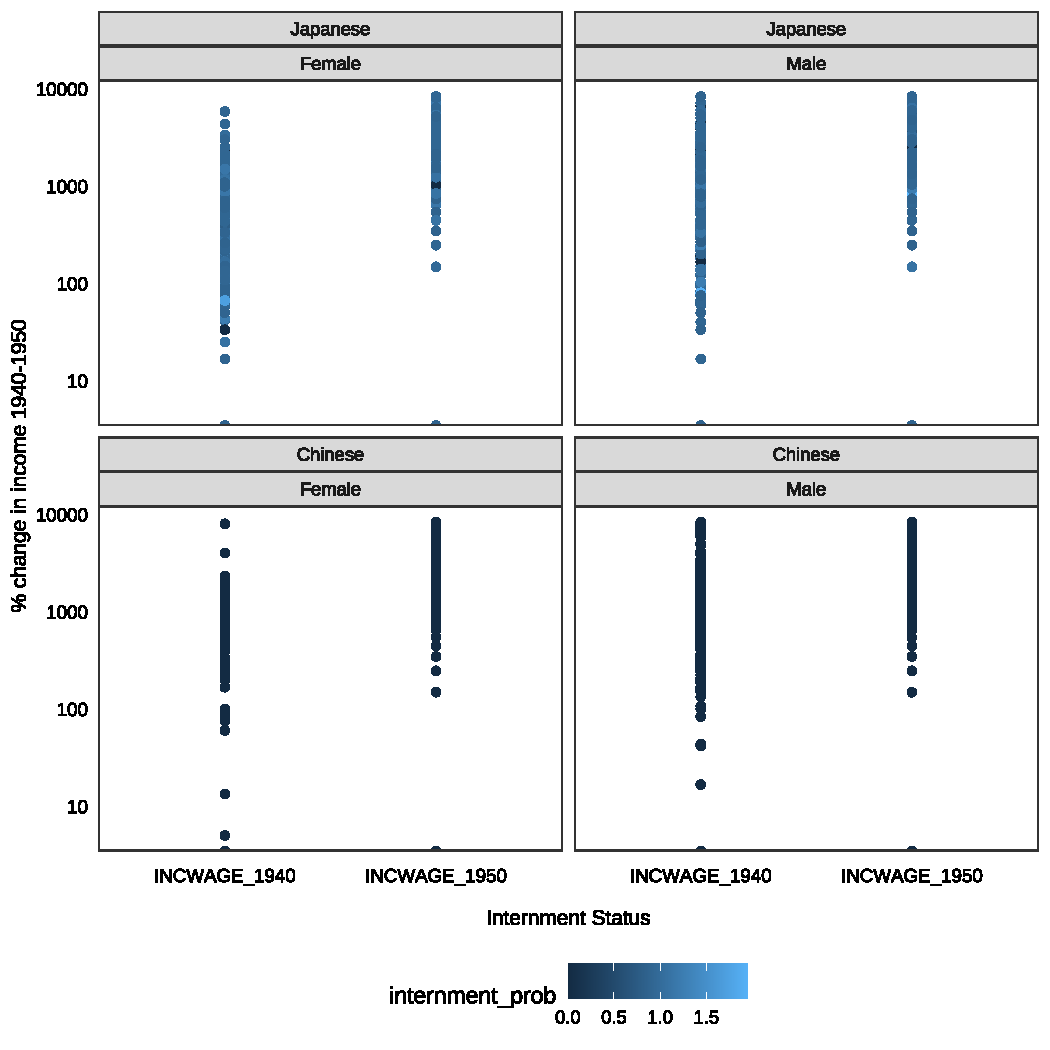
\includegraphics[width=\textwidth]{../figures/INCWAGE_plot.pdf} \\
  \footnotesize
    \emph{Note:}
  Interned proportions are calculated as the number of internees from the county divided by the county's Japanese population in the 1940 full-count census.
  Counties in white had zero Japanese respondents in the 1940 census.
  The map on the below comes from the 1942 Western Defense Command's Final Report 
  % \citep{dewittjohnl.FinalReportJapanese1943}
  and shows in color the evacuation areas along the West Coast.
\end{figure}


Table \ref{tbl:reghet} shows the results of \ref{eq:mainreg}
broken down into separate subsamples.
Without accounting for sex at all in the original sample,
the effect of internment appears negative and statistically insignificant.
Columns (2) and (3) separate out this sample into men and women, respectively.
In the sample with only Japanese and Chinese men, 
there does not appear to be a significant effect of internment status on 1950 income.
However, for the sample with Japanese and Chinese women,
this effect is positive and significant at the 1\% level.

\begin{table}[htbp]
   \caption{\label{tbl:reghet} Internment income effect heterogeneities}
   \bigskip
   \centering
   \begin{tabular}{lccccc}
      \toprule
       & \multicolumn{5}{c}{Income in 1950}\\
                                   & All            & Male            & Female         & JM              & JF \\   
                                   & (1)            & (2)             & (3)            & (4)             & (5)\\  
      \midrule 
      Internment Status            & -76.05         & -83.67          & 132.1$^{***}$  & -26.61          & 196.4$^{**}$\\   
                                   & (45.60)        & (66.66)         & (13.65)        & (147.2)         & (71.33)\\   
      Age                          & -17.52$^{***}$ & 39.90$^{***}$   & -43.55$^{***}$ & 65.18$^{***}$   & -41.25$^{***}$\\   
                                   & (4.961)        & (7.969)         & (8.167)        & (9.087)         & (10.80)\\   
      Age square                   & -0.0053        & -0.5879$^{***}$ & 0.2729$^{***}$ & -0.8232$^{***}$ & 0.2289$^{**}$\\   
                                   & (0.0467)       & (0.0771)        & (0.0752)       & (0.0881)        & (0.1026)\\   
      Income in 1940               & 0.3155$^{***}$ & 0.2021$^{***}$  & 0.3344$^{***}$ & 0.1535$^{***}$  & 0.1910$^{***}$\\   
                                   & (0.0158)       & (0.0176)        & (0.0715)       & (0.0140)        & (0.0318)\\   
       \\
      Observations                 & 8,136          & 4,921           & 3,215          & 3,427           & 2,640\\  
      R$^2$                        & 0.08718        & 0.08390         & 0.07804        & 0.08074         & 0.07355\\  
      Within R$^2$                 & 0.05617        & 0.05126         & 0.04222        & 0.04392         & 0.03915\\  
       \\
      Education fixed effects      & $\checkmark$   & $\checkmark$    & $\checkmark$   & $\checkmark$    & $\checkmark$\\   
      State$_{1940}$ fixed effects & $\checkmark$   & $\checkmark$    & $\checkmark$   & $\checkmark$    & $\checkmark$\\   
      \bottomrule
   \end{tabular}
   
   \par \raggedright 
   This table reports the estimates of internment status on 1950 wages across different subsamples of the main linked sample. Column (1) includes Japanese and Chinese men and women, column (2) includes only Japanese and Chinese men, column (3) includes only Japanese and Chinese women, and column (4) includes only Japanese men.
\end{table}

These results seem to suggest that even though my earlier regressions
controlled for sex on the right-hand side,
it may be that internee women were driving the earlier results.
This is surprising, but as shown in figure \ref{fig:wageeffect},
both Japanese and Chinese women seem to have experienced increases in earnings
over this period.
This is potentially because of increased labor force participation by women
during World War II carrying over into 1950.
Even considering this broad pattern,
Japanese internee women still seem to do better than other women in this sample.

Columns (4) and (5) further restrict the sample to only Japanese men
and Japanese women.
The internment status coefficient for men remains insignificant,
but the coefficient for women is even larger.
Because this sample is smaller than the overall sample,
there are fewer observations with which to estimate the main coefficient.
Despite the lower power, the positive estimated effect for Japanese women remains higher.

If Japanese experienced different levels of discrimination 
than Chinese after the war,
then it might be possible that in the regressions 
which include them in the control group,
the coefficient on internment status is biased downward.
By including Japanese in columns (4) and (5),
the control group comprises only those Japanese 
who lived in counties unaffected by internment
and who would have experienced arguably similar levels of discrimination
to the interned Japanese.
